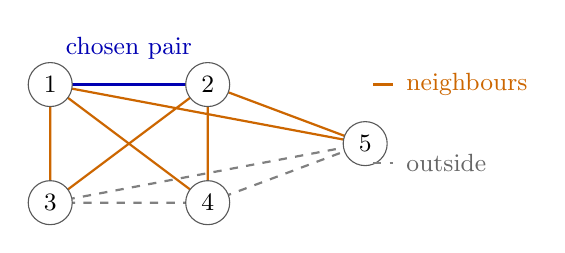
\begin{tikzpicture}[x=1cm,y=1cm]
\coordinate (a) at (0,1.5); \coordinate (b) at (2,1.5);
\coordinate (c) at (0,0); \coordinate (d) at (2,0); \coordinate (e) at (4,0.75);
\draw[blue!70!black,line width=1.3pt] (a)--(b);
\draw[orange!80!black,thick] (a)--(c) (a)--(d) (a)--(e) (b)--(c) (b)--(d) (b)--(e);
\draw[black!50,dashed,thick] (c)--(d) (c)--(e) (d)--(e);
\foreach \pt/\lab in {a/1,b/2,c/3,d/4,e/5}{\node[circle,fill=white,draw=black!65,inner sep=3pt,font=\small] at (\pt) {$\lab$};}
\node[blue!70!black,font=\small,above] at (1,1.7) {chosen pair};
\node[orange!80!black,font=\small,anchor=west] at (4.4,1.5) {neighbours};
\node[black!60,font=\small,anchor=west] at (4.4,0.5) {outside};
\draw[orange!80!black,thick] (4.1,1.5)--(4.35,1.5);
\draw[black!50,dashed,thick] (4.1,0.5)--(4.35,0.5);
\end{tikzpicture}
